%% ma: L12-B01-0005
%% lop: 12
%% chuong: 1
%% bai: 1
%% dang: 12.1.3
%% loai: TN4
%% muc: NB
%% dap_an: "C"
%% nguon: "(NBV)-ĐỀ SỐ 3-MỖI NGÀY 1 ĐỀ THI 2025.pdf (D03, MỖI NGÀY 1 ĐỀ - Đề số 3), Phần I Câu 1"
%% kien_thuc: "Bài 1 (điểm cực trị, đọc từ bảng biến thiên)"
%% trang_thai: chinh-thuc
%% ghi_chu: "Bảng biến thiên đề gốc mâu thuẫn: hàng f'(x) ghi dấu - 0 + + 0 - không khớp các mũi tên của hàng f(x) (giảm, tăng, giảm, tăng); đã dựng lại hàng dấu theo các mũi tên: - 0 + 0 - 0 +. Đáp án gốc C đúng. Giáo viên duyệt gộp dạng 12.1.5 vào 12.1.3 (10/10/2026)"
\begin{ex}
Cho hàm số $y=f(x)$ có bảng biến thiên như sau:
\begin{center}
\begin{tikzpicture}
  \tkzTabInit[lgt=1.5,espcl=2.3]{$x$/.8,$f'(x)$/.8,$f(x)$/2}{$-\infty$,$-1$,$1$,$3$,$+\infty$}
  \tkzTabLine{,-,0,+,0,-,0,+,}
  \tkzTabVar{+/$+\infty$,-/$0$,+/$3$,-/$0$,+/$+\infty$}
\end{tikzpicture}
\end{center}
Số điểm cực trị của hàm số đã cho là
\choice{$1$}{$2$}{\True $3$}{$4$}
\loigiai{Từ bảng biến thiên, $f'(x)$ đổi dấu khi qua $x=-1$, $x=1$ và $x=3$ nên hàm số có $3$ điểm cực trị (cực tiểu tại $x=-1$ và $x=3$, cực đại tại $x=1$).}
\end{ex}
